
\begin{document}

\chapter{Introduction}

\label{chapter:introduction}

People detection and tracking in realtime are essential in surveillance, interactive systems, medical imaging, and humanoid robotics.

The current project proposes an algorithm for tracking people with multiple Kinects which resolves the problem of occlusion.

\section{Problem Statement}
\label{sec:introduction_problem_statement}

The task of detecting and tracking moving targets is non-trivial. There are many sources of tracking errors, including raw sensor data noise, illumination levels, changing backgrounds, and occlusion. Real-world environments are unpredictive and complex, thus making the task much harder. The system attempts to solve the problme of occlusion with multiple Kinects.

Occlusion occurs when the tracked target is masked by other objects in the scene. The masked target would not exist in the field of view of one or more cameras. If a person were occluded, his precise joint positions and movements would be unknown. Resolving the problem of occlusion would provide any tracking system with more spatial and physiological information about the tracked people.

There are two types of occlusions: static and dynamic. They are defined as:

\begin{description}
  \item[Static occlusion] Occlusion caused by stationary objects in the environment 
  \item[Dynamic occlusion] Occlusion caused by people interactions in the environment
\end{description}

The project aims to resolve both types of occlusion.

A simple instance of the problem is illustrated in Figure \ref{fig:occlusion_problem}. In the figure, both skeletons are invisible to the front Kinect but visible to the side Kinect. They are occluded by the red obstacle. When they step out of the obstacle into the views of both Kinects, the system should merge the skeletons of the same person from different perspectives. The main objective of the project is to avoid occlusion by extending the field of view of the system. The proposed algorithm would combine depth sensor information from multiple Kinects to achieve this goal.

\begin{figure}[!h]
  \centering
  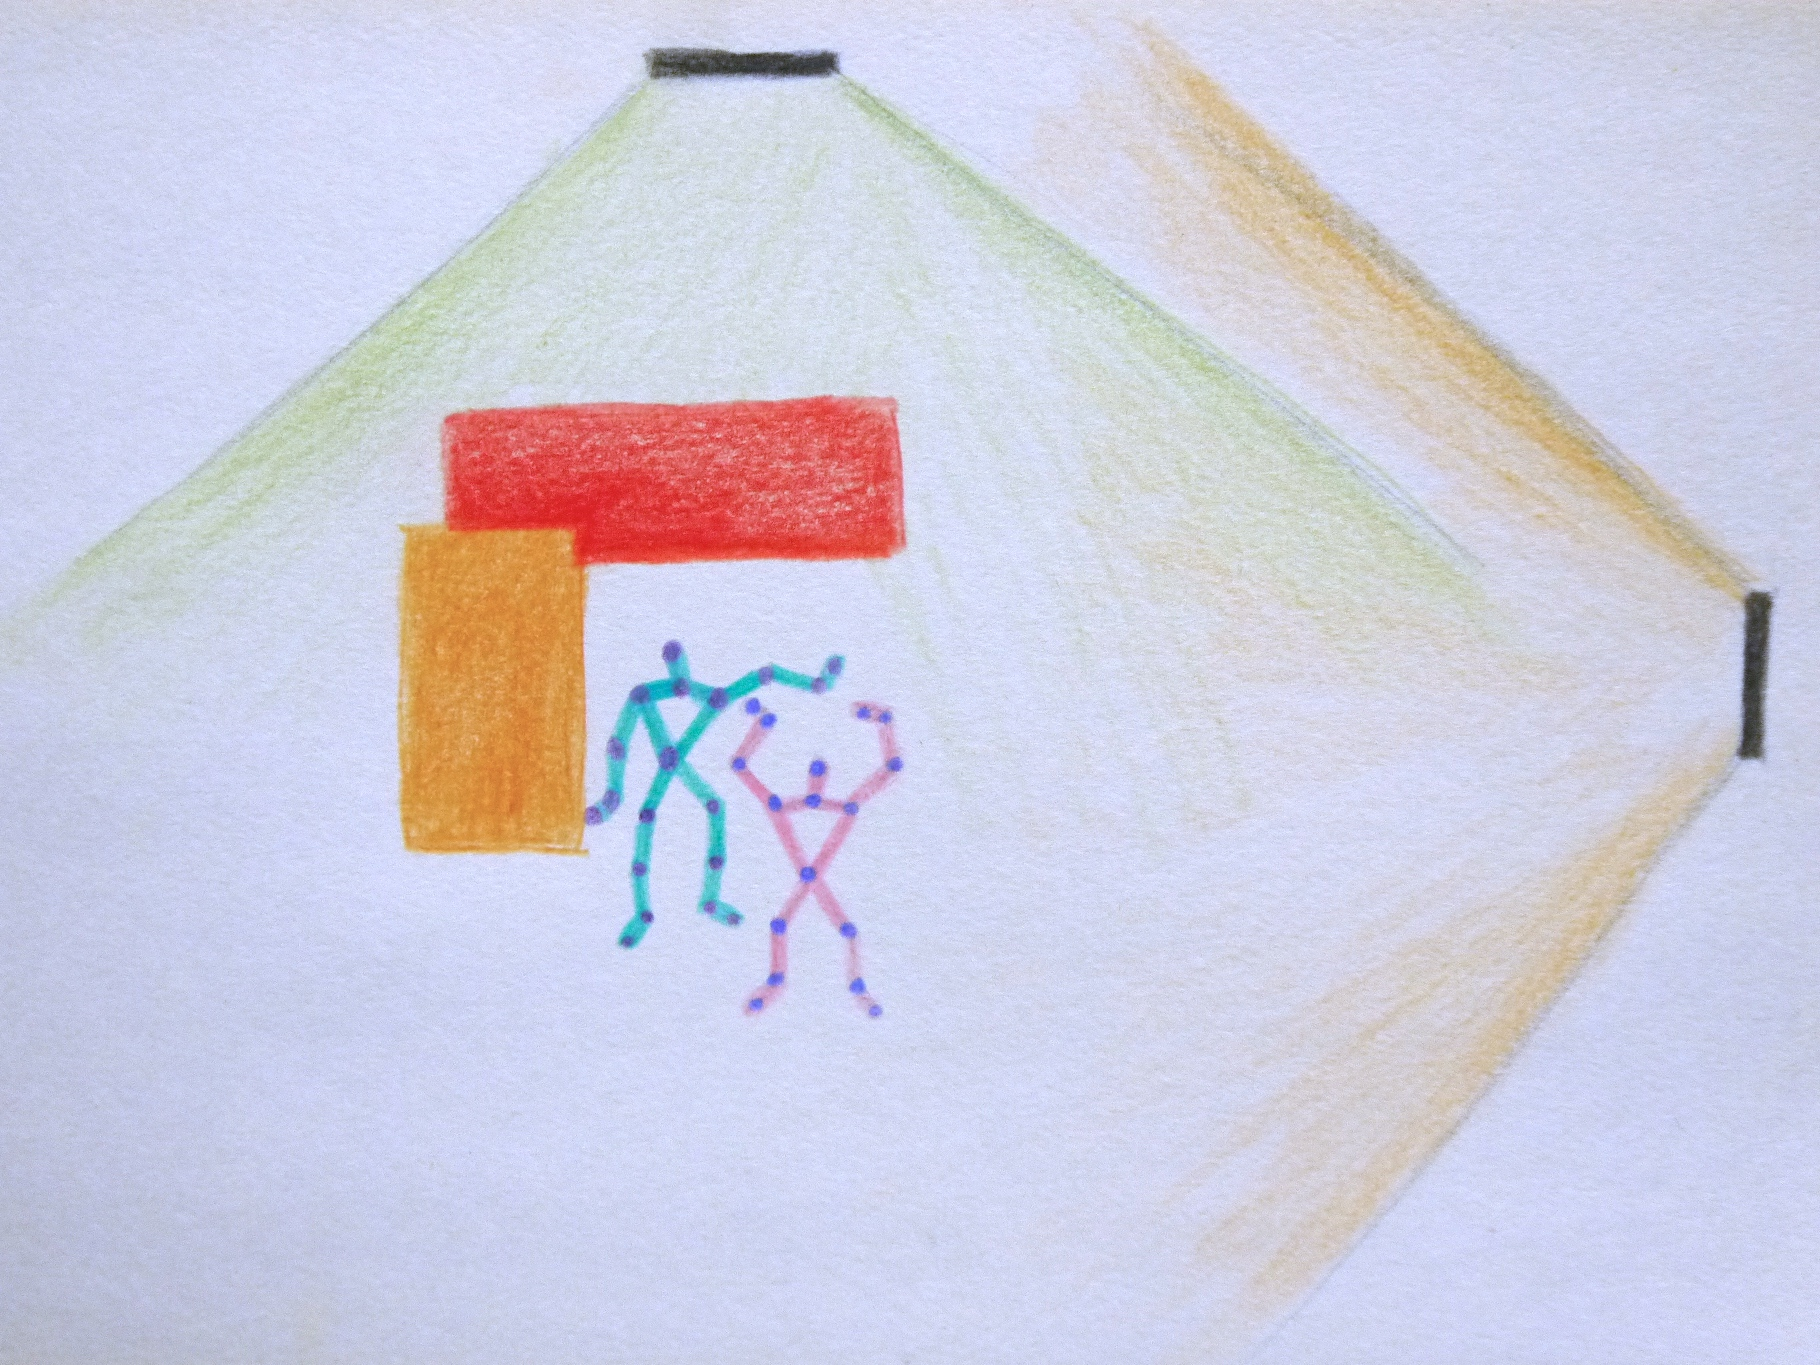
\includegraphics[width=0.8\linewidth]{figs/occlusion_problem}
  \caption{The occlusion problem}
  \label{fig:occlusion_problem}
\end{figure}

\section{Contributions}
\label{sec:introduction_contributions}

The contributions of the current work are\ldots

\begin{enumerate}
  \item Replicate, validate, and extend current research
  \item A Kinect BodyFrame serialization library
  \item A Kinect client-server framework
  \item Track people with multiple Kinects
  \item Display tracking skeletons from different Kinects fields of view
  \item Integrate joints information from multiple Kinects to resolve the occlusion problem
  \item User studies showing the strengths and weaknesses of the current system
\end{enumerate}

\section{Kinect}
\label{sec:introduction_kinect}

\textbf{TODO}

The specification and components. Include image Larger field of views. Give examples. Define field of view.

The complete API reference for Kinect v2 is accessible at {\url{https://msdn.microsoft.com/en-us/library/windowspreview.kinect.aspx}}.

Kinect Camera Space. The coordinates are 3D points (x, y, z), expressed in meters. The origin of the coordinate system at (0, 0, 0) is at the center of the Kinect's IR sensor. The x axis grows to the left of the Kinect, the y axis grows upward, and the z axis grows outward from the direction of the sensor.

\end{document}
